\problemname{Robottävling}

Du har byggt en robot till en robottävling. En av uppgifterna som roboten ska lösa går ut på att räkna antalet kuber i ett kvadratiskt rutnät. Rutnätet har $N$ rader och $N$ kolumner, och i varje ruta finns en stapel med $1$ till $5$ identiska kuber. Tyvärr är din robot inte särskilt bra på att samla information. Det enda den kan göra är att hitta höjden på den högsta stapeln i varje rad och kolumn. Du hade tänkt kompensera för detta genom att göra roboten väldigt smart. Skriv ett program som, givet informationen roboten samlade in, räknar ut det minsta och det största möjliga antalet kuber i rutnätet.

\section*{Indata}
På första raden står ett heltal $N$, antalet rader och kolumner i rutnätet. På andra raden står $N$ heltal $r_i$ $(1 \leq r_i \leq 5)$, höjden av högsta stapeln i rad $i$. På tredje raden står $N$ heltal $c_i$ $(1 \leq c_i \leq 5)$, höjden av högsta stapeln i kolumn $i$. Det är garanterat att det inte finns några motsägelser i indatan, det vill säga det kommer alltid att finnas minst en giltig utplacering av kuber som ger de givna värdena.
\section*{Utdata}
Programmet ska skriva ut två heltal: det minsta möjliga och det största möjliga totala antal kuber i rutnätet.


\section*{Poängsättning}
För testfall värda $20$ poäng gäller att $N=3$  och du behöver bara få rätt på det största antalet kuber. \\
För testfall värda $20$ poäng gäller att  $5\le N\le 10$   och du behöver bara få rätt på det största antalet kuber.\\
För testfall värda $20$ poäng gäller att  $N=3$.  \\
För testfall värda $40$ poäng gäller att  $5 \le N \le 10.$ \\

\section*{Exempelförklaring}
\begin{figure}[!h]
  \centering
      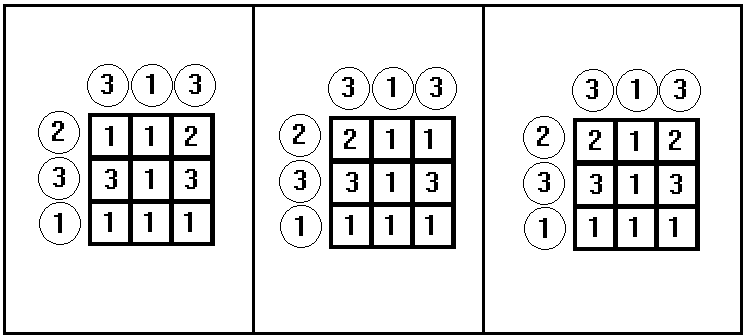
\includegraphics[width=.5\textwidth]{robotbild.png}
\end{figure}
Dessa tre är de enda möjliga konfigurationerna för det första exemplet. Båda de två första har totalt 14 kuber och den tredje har totalt 15 kuber. Svaret blir alltså att det minsta möjliga totala antalet kuber är 14, och det största möjliga är 15.
